%% LyX 2.0.3 created this file.  For more info, see http://www.lyx.org/.
%% Do not edit unless you really know what you are doing.
\documentclass[english]{article}
\usepackage[T1]{fontenc}
\usepackage[latin9]{inputenc}
\usepackage{geometry}
\geometry{verbose,tmargin=0.75in,bmargin=0.75in,lmargin=0.75in,rmargin=1in}
\usepackage{graphicx}

\makeatletter

%%%%%%%%%%%%%%%%%%%%%%%%%%%%%% LyX specific LaTeX commands.
%% Because html converters don't know tabularnewline
\providecommand{\tabularnewline}{\\}

\makeatother

\usepackage{babel}
\begin{document}
\thispagestyle{empty}

\begin{tabular*}{1\textwidth}{@{\extracolsep{\fill}}lr}
\textbf{ID:} 03 & \textbf{Collaborator \#1:} Last Name, First Name\tabularnewline
\textbf{Name:} Al-Naji, Nader & \textbf{Collaborator \#2:} Last Name, First Name\tabularnewline
\hline 
\end{tabular*}

\medskip{}


\begin{center}
\begin{Large}\textbf{Solution to HW 7, Problem 1}\end{Large}
\par\end{center}

\begin{center}
\begin{large}\textbf{COS 340 - Spring 2012}\end{large}
\par\end{center}

\bigskip{}


% Begin sol%
Suppose there are six people at a party. Prove that there are always three of them so that every two know each other (or) no two know each other.
\newline
\newline
In other words, let $G$ be a complete graph on $six$ vertices. Let the edges of $G$ be colored with two colors: red or blue. For any such coloring, prove that there is always a monochromatic triangle, ie: three vertices joined to each other by red edges (or) three vertices joined to each other by blue edges.
\newline
\newline
Label the vertices $a, b, c, d, e, f$. Consider vertex $a$. This vertex is connected to every other vertex in the graph by an edge and therefore has degree $5$. Moreover, no matter how we color these $5$ outgoing edges, it is clear that more than half of them will have the same color. That is, at least three of these outgoing edges will be either all blue or all red. Having noted this, say that three of them are some color, say red. Further, say the adjacent vertices these three edges lead to are $b, c, d$; it should be clear we can do this without loss of generality. So edges $a-b, a-c, a-d$ are all red. Now we consider coloring the edges $b-c, b-d, c-d$. In order to prevent a monochromatic triangle from being formed between these three vertices, we must color each edge between these vertices the opposite color, blue. But this forms a monochromatic triangle since $b-c, b-d, c-d$ form a triangle. Thus we have a contradiction. Note that we could have done this with any vertex, not just $a$ because the graph is complete and therefore symmetric with respect to each vertex. Further, note we can choose any three adjacent edges to the starting vertex for the second part and the proof will still hold. Thus, in general, no matter how we choose to color $K_6$, there will always be a monochromatic triangle.
\newline
\newline
Let $H$ be a complete graph on $five$ vertices. Show that the edges of $H$ can be colored with two colors (red, blue) without monochromatic triangles.
\newline
\newline
The following is a $2-coloring$ of $K_5$ without monochromatic triangles:
\newline
\newline
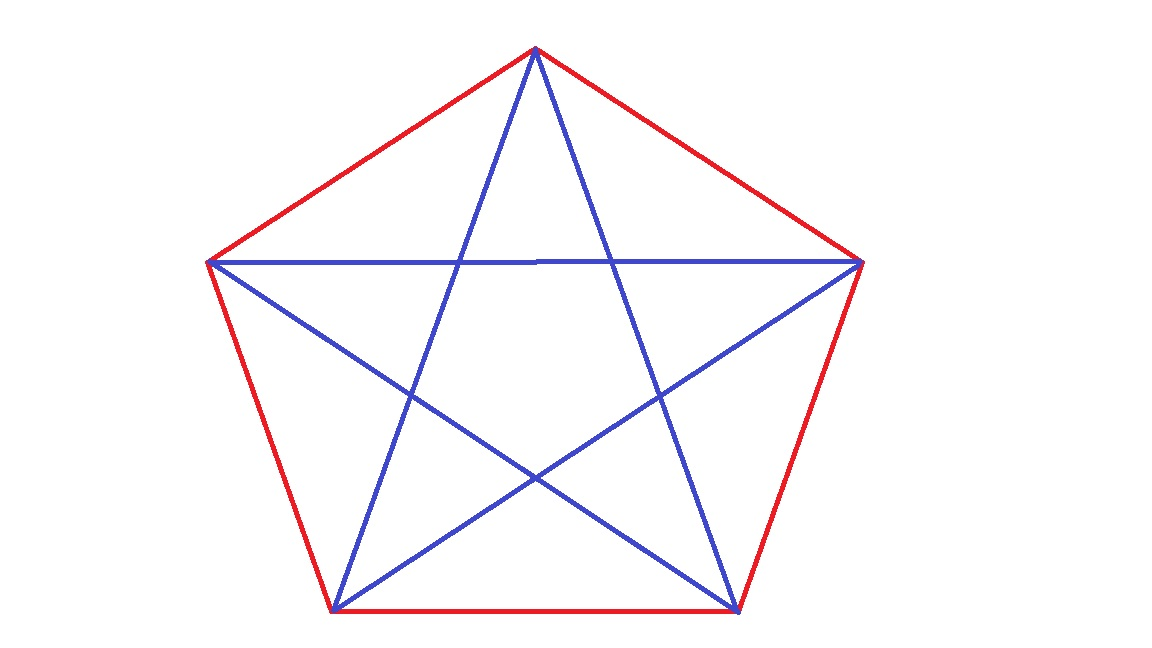
\includegraphics[scale=0.5]{myfig.jpg}
% End sol%

\pagebreak{}

\thispagestyle{empty}

\begin{tabular*}{1\textwidth}{@{\extracolsep{\fill}}lr}
\textbf{ID:} 03 & \textbf{Collaborator \#1:} Last Name, First Name\tabularnewline
\textbf{Name:} Al-Naji, Nader & \textbf{Collaborator \#2:} Last Name, First Name\tabularnewline
\hline 
\end{tabular*}

\medskip{}


\begin{center}
\begin{Large}\textbf{Solution to HW 7, Problem 2}\end{Large}
\par\end{center}

\begin{center}
\begin{large}\textbf{COS 340 - Spring 2012}\end{large}
\par\end{center}

\bigskip{}


% Begin sol%
Let $G(A, B, E)$ be a bipartite graph such that $|A| = |B| = 3$. It has all possible edges between $A$ and $B$, ie, it has nine edges. It is a simple graph with no self-loops or multi-edges. This graph is called $K_{3,3}$. Prove that $K_{3,3}$ is not planar.
\newline
\newline
First, we consider the minimum number of edges each face of $K_{3,3}$ can have surrounding it. A face is made whenever we have a cycle in the graph. The minimum number of edges each face can have surrounding it cannot be one since $K_{3,3}$ has no self-loops. This number also cannot be two since the graph is simple and a loop between two vertices would require a multi-edge, which simple graphs don't have. This number also cannot be three. To see this, simply consider that, starting from a vertex in $A$ or $B$, we cannot get back to a vertex in the set we started from without making an even number of hops, since the graph is bipartite. In other words, it should be clear that if we start on a vertex in $A$, after traversing one edge we will be in $B$, after traversing two edges we will be back in $A$ and, therefore, after traversing three edges, we will have to be back in $B$ since, in a bipartite graph, all the edges lead to a vertex in the opposite set of vertices. Thus, since on the third hop we will be in a set different from the set we started in, we cannot make a loop in three hops and, therefore, any face in $K_{3,3}$ must be surrounded by at least four edges. This gives us that the number of face boundaries is $b \geq 4f$ since every face must contribute at least four boundaries by the preceding argument. Further, since each edge can contribute two boundaries, we get that: $2e \geq 4f \rightarrow e \geq 2f$ if $K_{3,3}$ is planar. 
\newline
\newline
Having noted this, now we compute the number of faces using Euler's formula and show that the above inequality leads to a contradiction. We have: $v + f = 2 + e \rightarrow f = 2 + e - v \rightarrow f = 2 + 9 - 6 \rightarrow f = 5$. So the number of faces $K_{3,3}$ has is $5$ if it is planar. This leads the inequality above to suggest that $e \geq 2f = 10$ if $K_{3,3}$ is planar. But we know that $e = 9 < 10$ and thus we have a contradiction proving that $K_{3,3}$ is not planar.
% End sol%

\pagebreak{}
\thispagestyle{empty}

\begin{tabular*}{1\textwidth}{@{\extracolsep{\fill}}lr}
\textbf{ID:} 03 & \textbf{Collaborator \#1:} Last Name, First Name\tabularnewline
\textbf{Name:} Al-Naji, Nader & \textbf{Collaborator \#2:} Last Name, First Name\tabularnewline
\hline 
\end{tabular*}

\medskip{}


\begin{center}
\begin{Large}\textbf{Solution to HW 7, Problem 3}\end{Large}
\par\end{center}

\begin{center}
\begin{large}\textbf{COS 340 - Spring 2012}\end{large}
\par\end{center}

\bigskip{}


% Begin sol%
A random graph is a graph whose edges are chosen randomly from a specified distribution. Various random graph models have been used to understand properties of social networks, the world-wide-web, and so on. In this problem, we will study a simple example of a random graph model and investigate the existence of cliques, ie subgraphs where all pairs of vertices are connected by an edge. 
\newline
\newline
Let $G_n$ be a random graph on $n$ nodes where each of the $n \choose 2$ possible edges is included in the set with probability $1/2$, independently of the other edges.
\newline
\newline
\textbf{1. Show that with high probability, $G_n$ does not contain a clique of size $3 \lg n$.}
\newline
\newline
First, we compute the expected number of cliques in a graph of size $n$. Afterwards, we use Markov's inequality to show that $P(\mbox{number of cliques} \geq 1) \rightarrow 0$ as $n$ becomes large. Begin with computing the expectation:
\newline
\newline
First, note that for any particular set of $k$ vertices to be a clique, we need for all of the $k \choose 2$ edges to be filled in. The probability that each edge is filled in is $1/2$ and so we have:
\newline
\newline
$P(\mbox{a particular set of k vertices is a clique}) = (1/2)^{k \choose 2} = (1/2)^{k(k-1)/2}
\newline\rightarrow P(\mbox{any particular set of } 3\lg n \mbox{vertices is a clique}) = (1/2)^{(3 \lg n)(3\lg n-1)/2} = \frac{1}{2^{9\lg^2 n - 3 \lg n}/2} = n^{(3/2)(1-3\lg n)}$
\newline
\newline
Now, define an ordering over every distinct subset of $3 \lg n$ vertices (note that there are ${n} \choose {3 \lg n}$ such subsets), and define $I_k$ to be an indicator random variable that is $1$ if the $k_{th}$ set of $3 \lg n$ vertices is a clique. Further, let $X_n$ be the number of cliques of size $3 \lg n$ in a random graph of $n$ nodes. Then, the expected number of cliques is simply the expectation over all of these indicators summed together and, noting that these indicators are all identically distributed, we have:
\newline
\newline
$E[X_n] = E[\sum\limits_{k=1}^{{n} \choose {3 \lg n}} I_k] = E[\sum\limits_{k=1}^{{n} \choose {3 \lg n}} I_1] = \sum\limits_{k=1}^{{n} \choose {3 \lg n}} E[I_1] =
{{n} \choose {3 \lg n}} E[I_1] = {{n} \choose {3 \lg n}} n^{(3/2)(1-3\lg n)}$.
\newline
\newline
Note how awesome linearity of expectation is. We now have an expression for the expectation; all that is left is simply to show that this expression tends to zero as $n$ becomes large:
\newline
\newline
$\lim\limits_{n\rightarrow\infty}{{n} \choose {3 \lg n}} n^{(3/2)(1-3\lg n)} = \lim\limits_{n\rightarrow\infty}\frac{(n)(n-1)(n-2)...(n-(3\lg n - 2))(n - (3 \lg n - 1))}{(3 \lg n)!} \frac{n^{3/2}}{n^{9/2 \lg n}} 
\newline= \lim\limits_{n\rightarrow\infty}\frac{n^{3 \lg n}(1)(1-1/n)(1-2/n)...(1-(3\lg n - 2)/n)(1 - (3 \lg n - 1)/n)}{(3 \lg n)!} \frac{n^{3/2}}{n^{9/2 \lg n}}
\newline= \lim\limits_{n\rightarrow\infty}\frac{n^{3 \lg n}}{(3 \lg n)!} \frac{n^{3/2}}{n^{9/2 \lg n}} = \lim\limits_{n\rightarrow\infty}\frac{1}{(3 \lg n)!} \frac{n^{3/2}}{n^{3/2 \lg n}} = 0
\rightarrow \lim\limits_{n\rightarrow\infty} E[X_n] = 0$.
\newline
\newline
Finally, having shown that the expected number of cliques of size $3 \lg n$ tends to zero as $n$ becomes large, we use Markov's inequality to show that this implies that the probability that $G_n$ contains a clique of size $3 \lg n$ tends to zero as $n$ grows large:
\newline
\newline
$P(X_n \geq a) \leq E[X_n]/a \rightarrow P(X_n \geq 1) \leq E[X_n] \rightarrow \lim\limits_{n \rightarrow \infty} P(X_n \geq 1) \leq \lim\limits_{n \rightarrow \infty} E[X_n]
\rightarrow \lim\limits_{n \rightarrow \infty} P(X_n \geq 1) \leq 0 \rightarrow \lim\limits_{n \rightarrow \infty} P(X_n \geq 1) = 0$.
\newline
\newline
Thus, the probability that $G_n$ contains a clique of size $3 \lg n$ becomes vanishingly small as $n$ becomes large.
\newline
\newline
\textbf{2. Show that with high probability, $G_n$ contains a clique of size $(1/2)\lg n$.}
\newline
\newline
The probability that any vertex connects to any other vertex is $1/2$. If we have any particular set of $k$ vertices, note that the probability that any given vertex not in this set is connected to all the vertices in this set is $1/2^k$. Now, consider an algorithm that finds a clique of size $K$ if it exists. This algorithm starts with an empty set of vertices and, at each step $k$, adds a vertex to this set if (it isn't currently in the set) AND (it is connected to each of the $k-1$ vertices currently in the set). If this algorithm succeeds, then clearly there exists a clique of size $K$ in the graph. We now compute the probability that this algorithm succeeds on a graph of size $n$ looking for a clique of size $1/2 \lg n$ and show that this probability tends to $1$ as $n$ becomes large. 
\newline
\newline
First, note that in order for the algorithm to succeed, every step in the algorithm has to succeed. Thus, we can write the probability that the algorithm succeeds as follows. Let $S_k$ be  the event that the algorithm succeeds at step $k$:
\newline
\newline
$P(\mbox{algorithm succeeds}) = P(S_1, S_2, ..., S_K) = P(S_1 | S_2, ..., S_K)P(S_2 | S_3, ..., S_K)...P(S_K) 
\newline= P(S_1)P(S_2|S_1)P(S_3|S_2)...P(S_K|S_{K-1})$.
\newline
\newline
Note that above we used the fact that whether or not the algorithm succeeds at the $k_{th}$ step is dependent only on whether or not the algorithm succeeded at the $(k-1)_{th}$ step. Now, before we continue, note that the probability that the algorithm succeeds at the $(k+1)_{th}$ step given that it succeeded at the $k_{th}$ step is equal to $1 - P(\mbox{algorithm fails at the } (k+1)_{th} \mbox{ step})$. Further, the probability that the algorithm fails at the $(k+1)_{th}$ step given it made it through the $k_{th}$ step is simply the probability that none of the $n-k$ vertices connect to the current clique of size $k$, or simply: $P(S_k) = 1 - (1-1/2^{k})^{n-k}$.  So, to summarize, now that we know that the probability that the algorithm gets to the end of $K$ iterations can be broken down into the probability that it gets through each individual iteration, and now that we have the probability that it gets through each individual iteration, we can finally write down the probability that the algorithm finds a clique of size $K$:
\newline
\newline 
$P(\mbox{algorithm succeeds}) = P(S_1)P(S_2|S_1)P(S_3|S_2)...P(S_K|S_{K-1}) = \prod\limits_{k=1}^{1/2 \lg n} 1 - (1-1/2^{k})^{n-k}$.
\newline
\newline
And now things get a little tricky. Because this product is difficult to evaluate, we note that we can exchange the inner terms with a smaller $k-independent$ probability and make the expression easier to manage while still being able to show that the original expression tends to one as $n \rightarrow \infty$. We do this by saying that this probability is greater than some easier-to-evaluate probability that still evaluates to one in the limit as follows:
\newline
\newline
$\prod\limits_{k=1}^{1/2 \lg n} 1 - (1-1/2^{k})^{n-k} \geq \prod\limits_{k=1}^{1/2 \lg n} 1 - (1-1/2^{(1/2 \lg n)})^{n-(1/2 \lg n)} = \prod\limits_{k=1}^{1/2 \lg n} 1 - (1 - 1/\sqrt{n})^{n - (1/2 \lg n)}
\newline= (1 - (1 - 1/\sqrt{n})^{n - (1/2 \lg n)})^{1/2\lg n}$.
\newline
\newline
Now we take the limit of this expression as $n \rightarrow \infty$ and show that it tends to one. First, we show that $(1 - 1/\sqrt{n})^{n - (1/2 \lg n)}$ tends to zero in the limit and then use this to show the whole expression tends to one:
\newline
\newline
$\lim\limits_{n \rightarrow \infty} (1 - 1/\sqrt{n})^{n - \lg \sqrt{n}}  = \lim\limits_{n \rightarrow \infty} \frac{((1 - 1/\sqrt{n})^{\sqrt{n}})^{\sqrt{n}}}{(1 - 1/\sqrt{n})^{\lg\sqrt{n}}} =  \lim\limits_{n \rightarrow \infty} \frac{(1/e)^{\sqrt{n}}}{(1 - 1/\sqrt{n})^{\lg\sqrt{n}}} \rightarrow 0/1 = 0$.
\newline
\newline
Note that we take it for granted that $(1 - 1/\sqrt{n})^{\lg\sqrt{n}}$ tends to one as $n \rightarrow \infty$. This can be shown using standard techniques from BC Calculus and so its proof is omitted here as it isn't terribly relevant. Additionally, note the use of the definition of $e^{-x}$ above to complete the limit evaluation.
\newline
\newline
Finally, having shown that the second term in the probability expression tends to zero as $n$ grows large, we complete the evaluation of the limit:
\newline
\newline
$\lim\limits_{n \rightarrow \infty} (1 - (1 - 1/\sqrt{n})^{n - (1/2 \lg n)})^{1/2\lg n} \rightarrow \lim\limits_{n \rightarrow \infty} (1 - 0)^{1/2\lg n} \rightarrow 1$.
\newline
\newline
Again, we take it for granted that an expression of the form $\lim\limits_{n \rightarrow \infty}(1 - 1/g(n))^{f(n)} \rightarrow 1$ for a particular choice of $g(n)$ and $f(n)$. While this is not true in general, we take it for granted that it is true in this case, omitting a simple proof using methods learned (and forgotten...) in BC Calculus. Thus, we have the result that we wanted.
\newline
\newline
To summarize, we have shown that (letting $X_n$ be the number of cliques of size $1/2 \lg n$ in a random graph of size $n$):
\newline
\newline
$\lim\limits_{n \rightarrow \infty} P(X_n \geq 1) \geq P(\mbox{algorithm described completes}) = \lim\limits_{n \rightarrow \infty} \prod\limits_{k=1}^{1/2 \lg n} 1 - (1-1/2^{k})^{n-k} 
\newline\geq \lim\limits_{n \rightarrow \infty} (1 - (1 - 1/\sqrt{n})^{n - (1/2 \lg n)})^{1/2\lg n} \rightarrow 1$.
\newline
\newline
Thus, having shown that the probability that there exists a clique of size $1/2 \lg n$ in a set of $n$ vertices tends to one as $n$ tends to infinity, we conclude that, with high probability, $G_n$ contains a clique of size $1/2 \lg n$ for large $n$.
\newline
\newline
% End sol%

\pagebreak{}

\thispagestyle{empty}

\begin{tabular*}{1\textwidth}{@{\extracolsep{\fill}}lr}
\textbf{ID:} 03 & \textbf{Collaborator \#1:} Last Name, First Name\tabularnewline
\textbf{Name:} Al-Naji, Nader & \textbf{Collaborator \#2:} Last Name, First Name\tabularnewline
\hline 
\end{tabular*}

\medskip{}


\begin{center}
\begin{Large}\textbf{Solution to HW 7, Problem 4}\end{Large}
\par\end{center}

\begin{center}
\begin{large}\textbf{COS 340 - Spring 2012}\end{large}
\par\end{center}

\bigskip{}


% Begin sol%
Let $G$ be a $3-regular$ plane graph such that every face of $G$ is either a pentagon (5 edges) or a hexagon (6 edges). The total number of vertices in $G$ is $v = 60$. Denote the total number of edges in $G$ by $e$, the total number of pentagons by $f_5$, and the total number of hexagons by $f_6$. 
\newline
\newline
1. Calculate $e$. 
\newline
\newline
This graph is $3-regular$ which means that every vertex has degree exactly three. It is a fact (since every edge contributes twice to the sum of the vertex degree as shown in class) that $\sum\limits_{v \in V}^{} deg_v = 2e$ so we have: $\sum\limits_{v \in V}^{} 3 = 2e \rightarrow (60)(3)/2 = e \rightarrow e = 90$.
\newline
\newline
2. Calculate the total number of faces $f = f_5 + f_6$.
\newline
\newline
Euler's formula for planar graphs is $v + f = 2 + e$. From this, we get: $f = 2 + e - v \rightarrow f = 2 + 90 - 60 \rightarrow f = 32$.
\newline
\newline
3. Use parts (1) and (2) to calculate $f_5$ and $f_6$.
\newline
\newline
The graph is planar and 3-regular so every edge is in the boundary of two faces. Further, if we know the number of pentagons and hexagons, we can count the number of boundaries in the embedded graph, divide this by two, and set it equal to the number of edges. Thus, we have two variables in two equations as follows:
\newline
\newline
$5 \cdot f_5 + 6 \cdot f_6 = 2e
\newline
f_5 + f_6 = f \rightarrow f_5 = f - f_6
\newline
\newline
\rightarrow 5f - 5\cdot f_6 + 6\cdot f_6 = 2e \rightarrow f_6 = 2e - 5 \cdot f \rightarrow f_6 = 180 - 5\cdot 32 = 20
\newline
\newline
\rightarrow f_6 = 20; \mbox{ } f_5 = 32 - 20 = 12$.
% End sol%

\pagebreak{}

\end{document}
